\section{Учет теплопроводности в материале}

Перенос тепла в материале стенки на достаточно малых временах может быть описан одномерной задачей:
\begin{subequations}
    \begin{align}
        \partial_t u &= a^2 \partial^2_x u\\
        \left(\partial_x u\right)(x = d) &= \varkappa q_{plasma}\\
        u(x = 0) &= T_0 \\
        u(t = 0) &= T_0 \\
        0 < x &< d \\
        t &> 0
    \end{align}
    \label{eq::heatcond_problem_decl}
\end{subequations}
$a^2 = \cfrac{\varkappa}{C_p\rho}$ --- коэффициент температуропроводности, $\varkappa$ --- коэффициент теплопроводности
Для вольфрама при $T = 1000$ К, параметры имеют значения:
\begin{subequations}
    \begin{align*}
        \varkappa = 118\text{ Вт/(м$\cdot$К)}\\
        \rho = 19.1\cdot 10^3\text{ кг/м$^3$}\\
        C_p = 144.5\text{ Дж/(кг$\cdot$ К)}
    \end{align*}
\end{subequations}

ПЛМ является выбросом плазмы из основного объёма реактора. Ввиду отличной проводимости \hl{сколько?порядка проводимости стали}, 
она ``вмораживает`` магнитные линии, осциллирующие с частотой порядка $10^8$ Гц~\cite{kirk2006evolution}. Осцилляции 
магнитного поля приводят к осцилляции электростатического потенциала. Принимая, что скорость ионов сохраняется, 
эти осцилляции могут представлены как осцилляции потенциала $V_f$.

Задача~\eqref{eq::heatcond_problem_decl} может быть решена методом линий\hl{цитата}.

Проводимость дебаевского слоя может быть описана значением импеданса~\cite{myra2015radio}:
\begin{equation}
    \cfrac{1}{z} = \cfrac{\langle JV\rangle}{\langle V^2\rangle} - \cfrac{i\omega\langle J\dot{V}\rangle}{\langle \dot{V}^2\rangle}
\end{equation}

\begin{figure}[H]
	\centering
	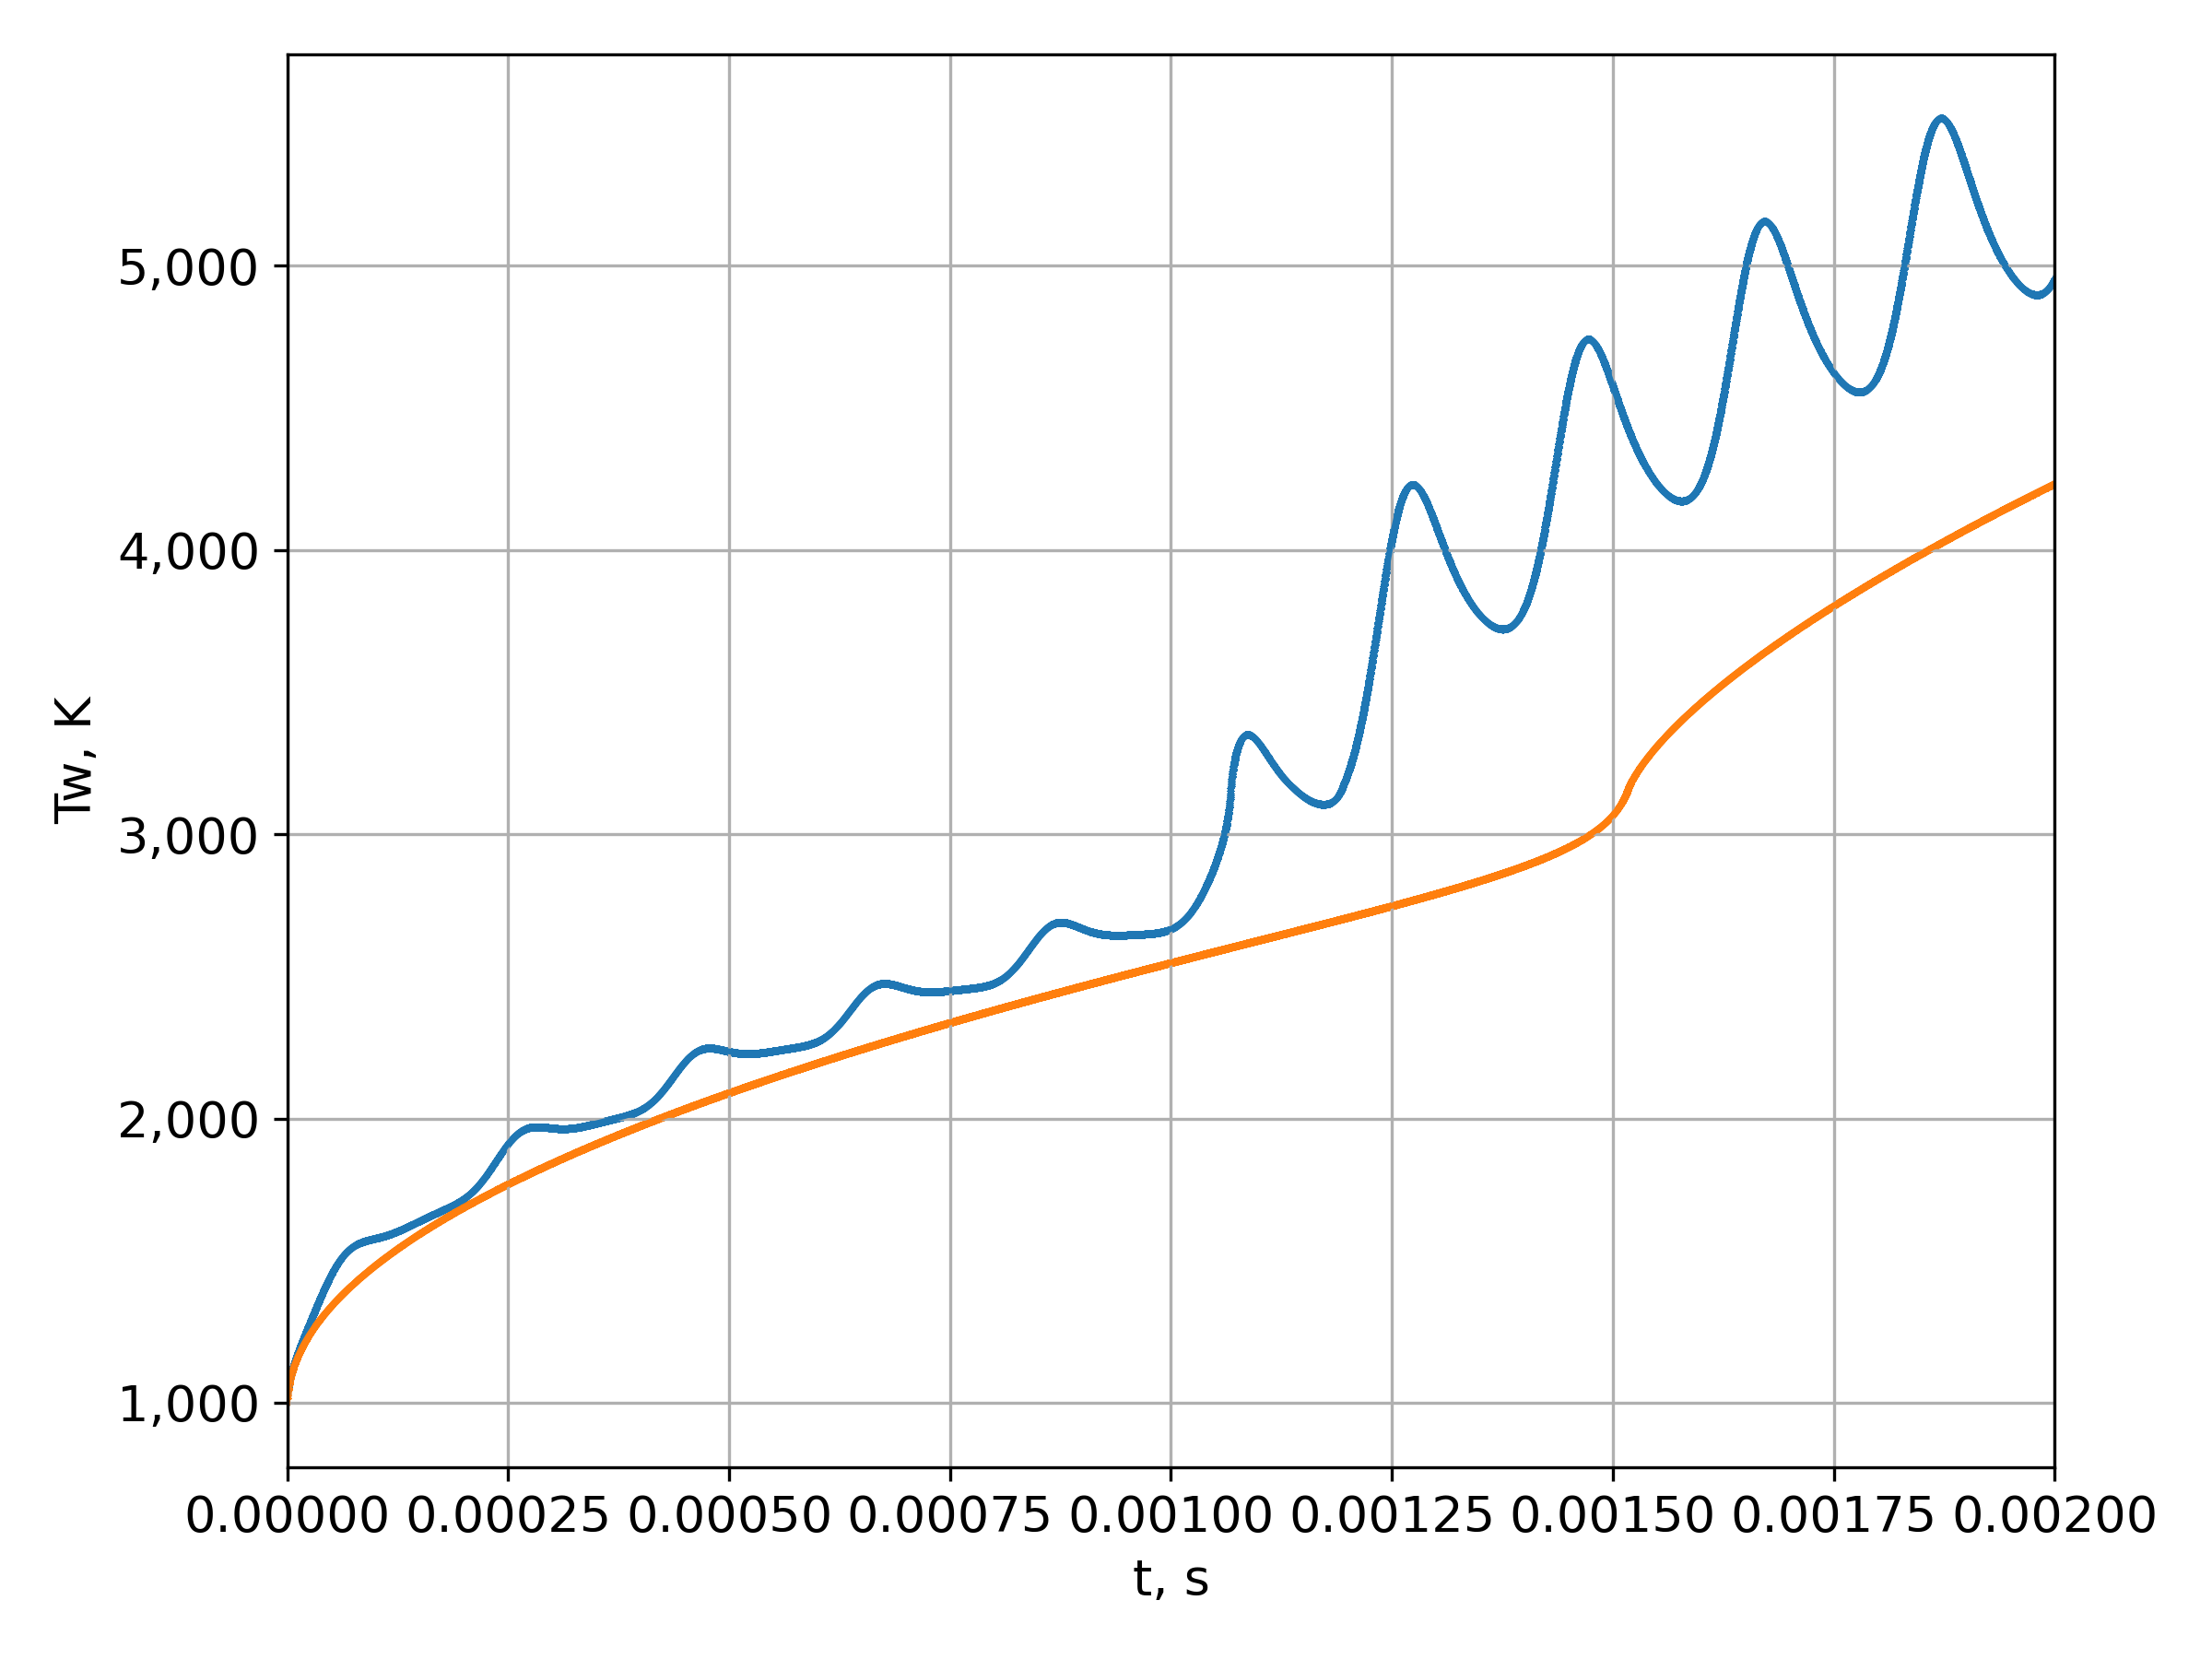
\includegraphics[width=0.7\linewidth]{material/omega10amp1.0/temperature_plot.png}
    \caption[]{Эволюция температуры поверхности плитки $T_s$}
    \label{pic::heatcond::omega10amp1.0::temperature_plot}
\end{figure}

\begin{figure}[H]
	\centering
	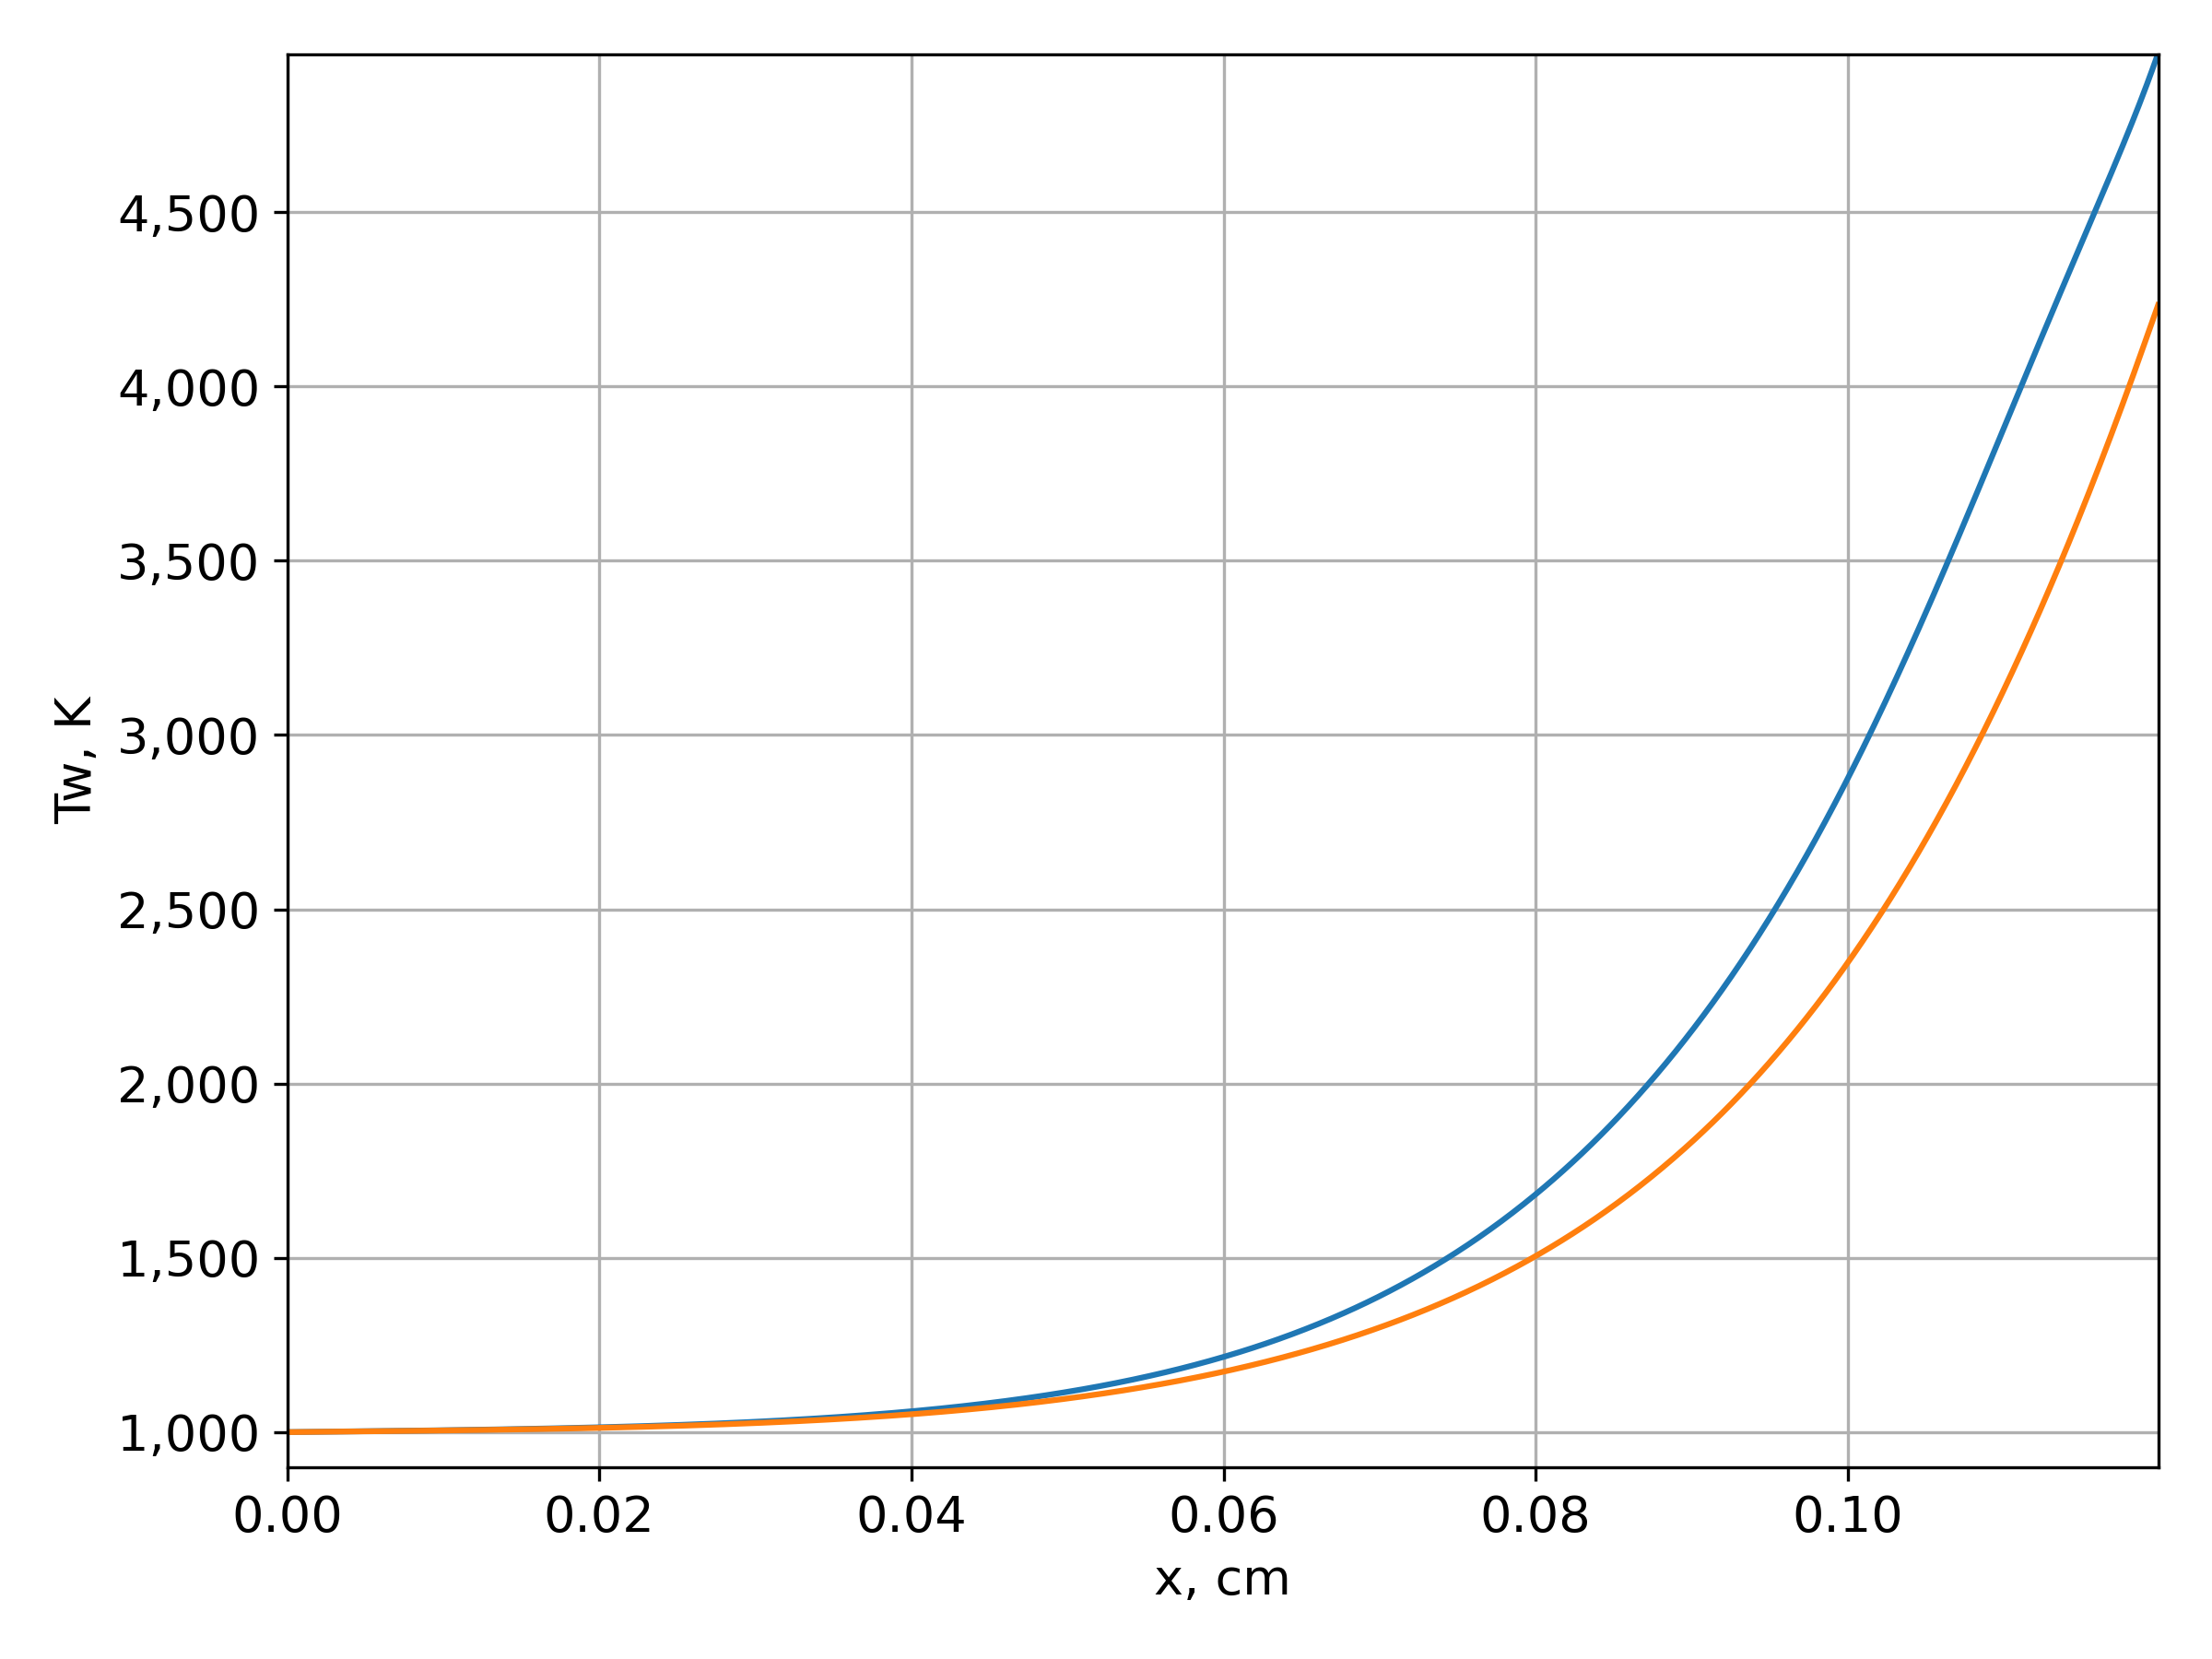
\includegraphics[width=0.7\linewidth]{material/omega10amp1.0/temperature_distribution_plot.png}
    \caption[]{Профиль температуры в плитке}
    \label{pic::heatcond::omega10amp1.0::temperature_distribution_plot}
\end{figure}
\begin{figure}[H]
	\centering
	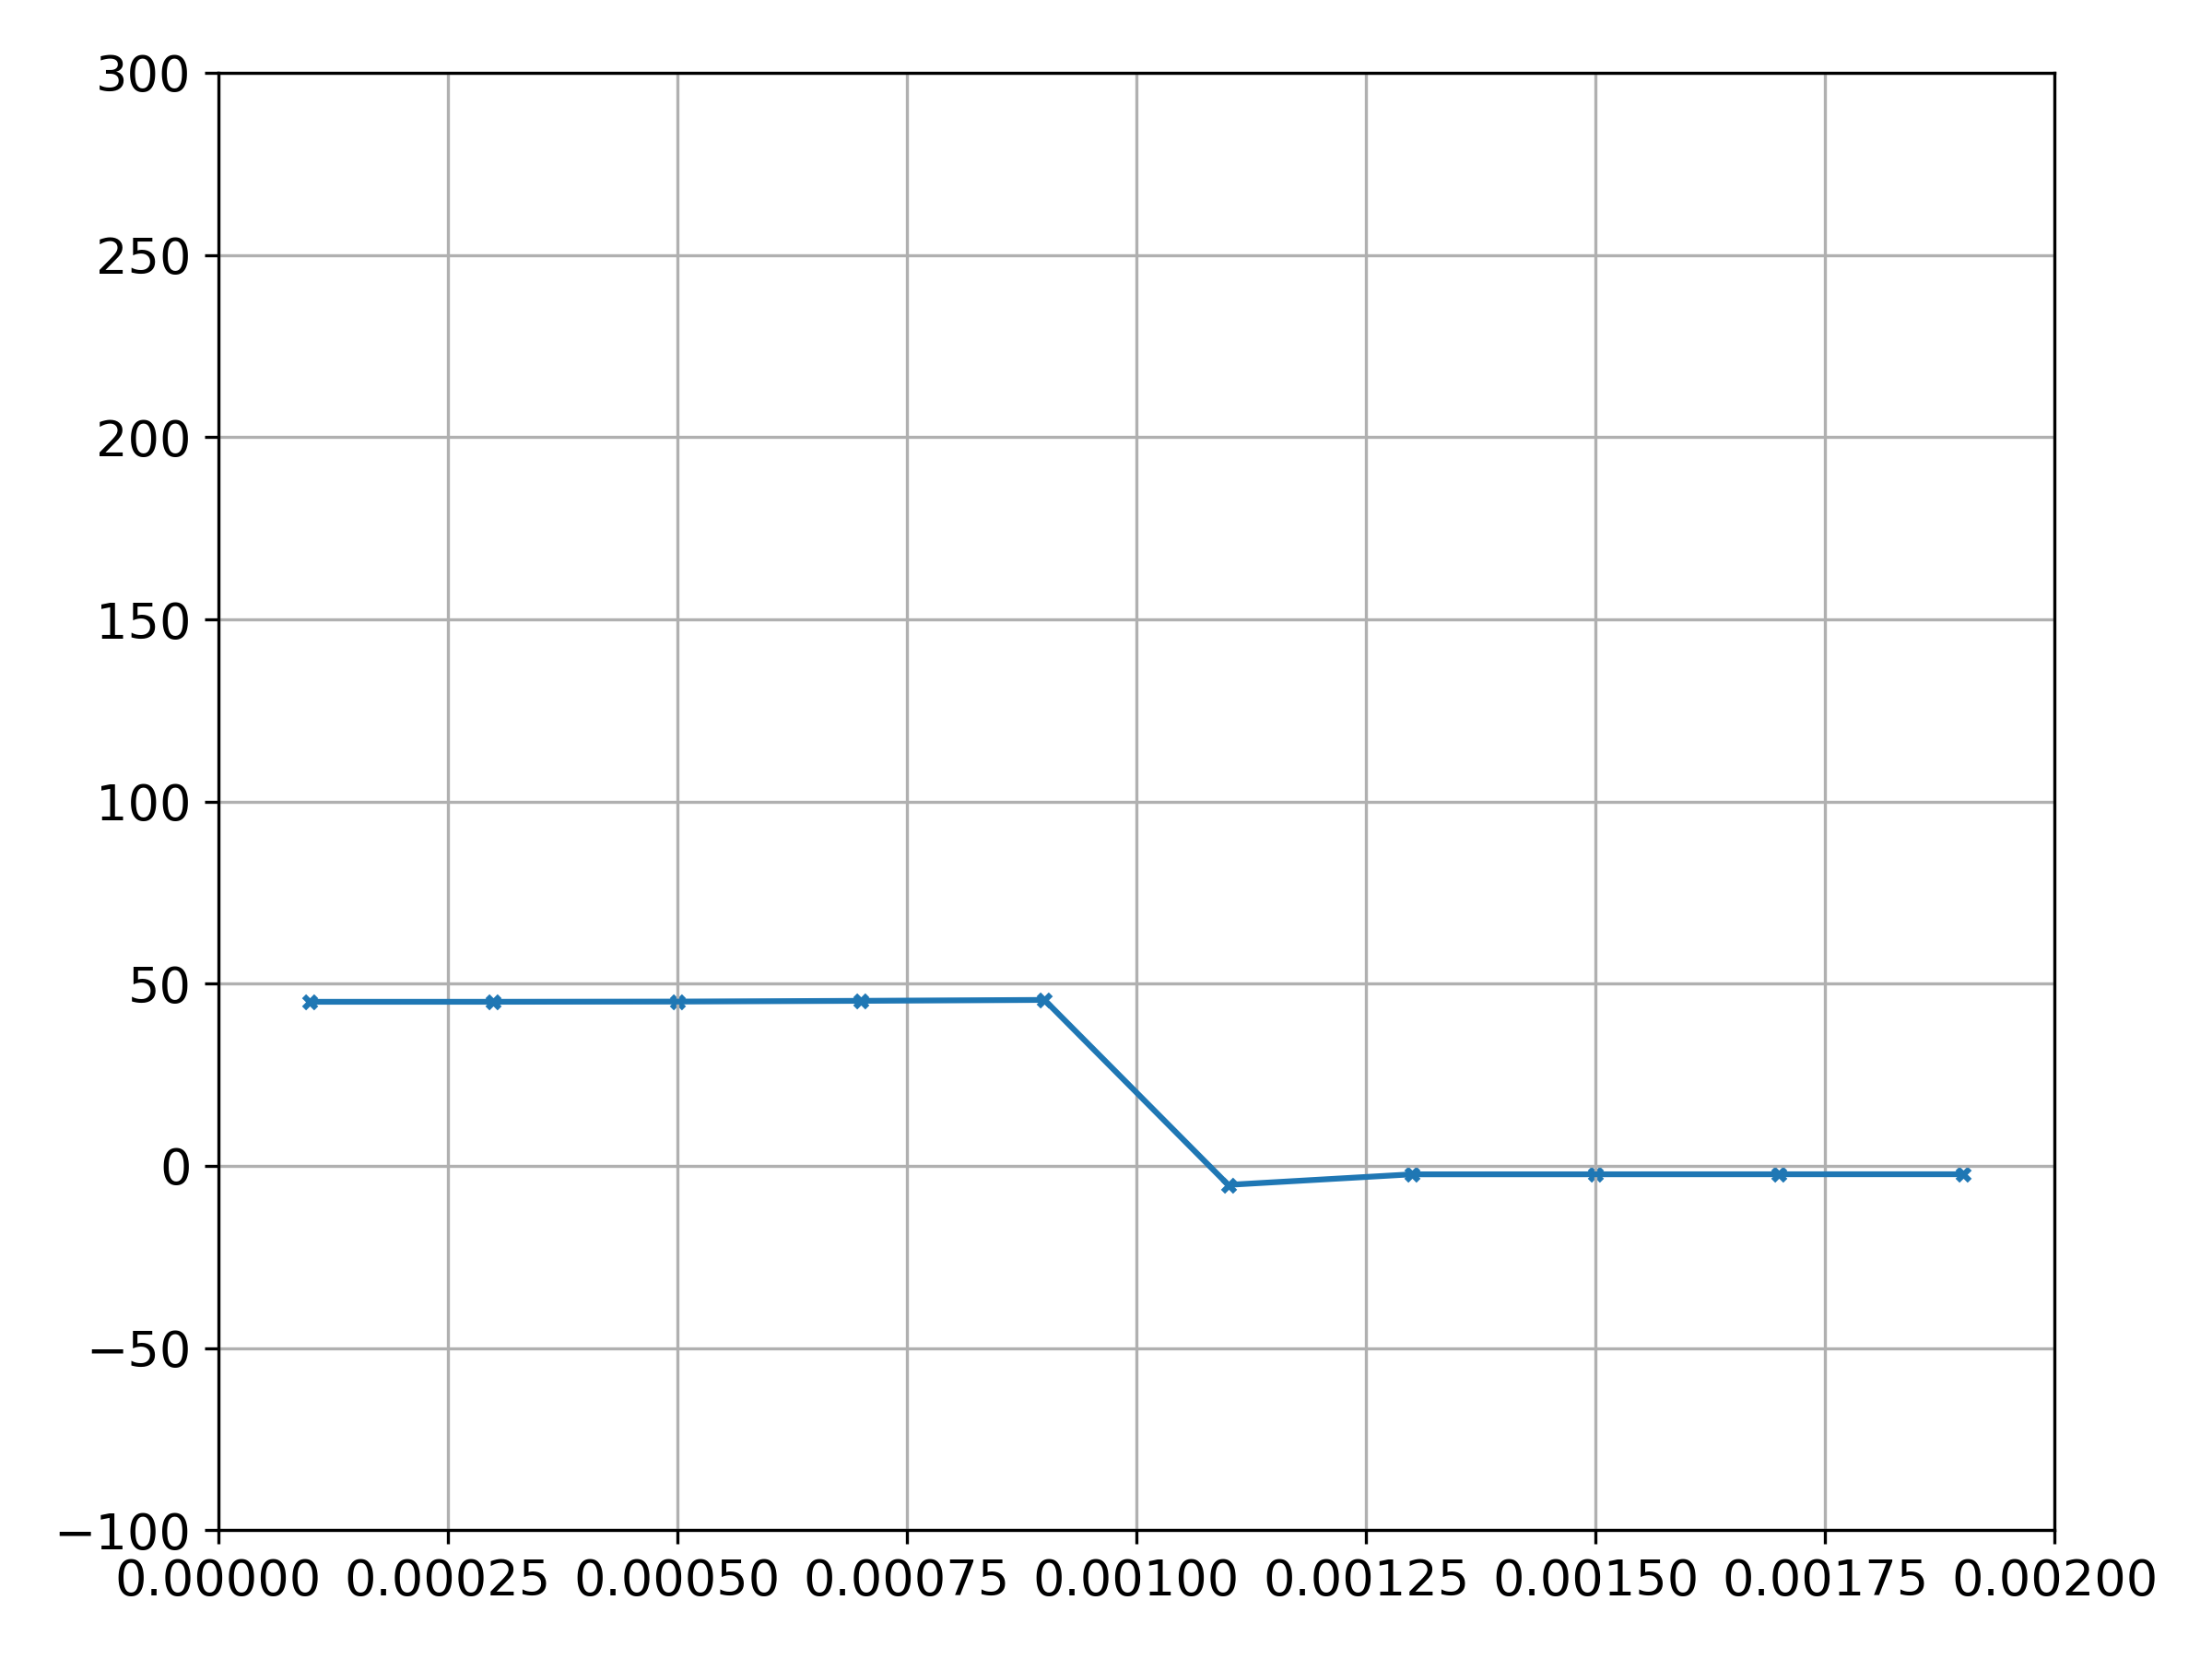
\includegraphics[width=0.7\linewidth]{material/z_plot.png}
    \caption[]{Эволюция резистивной части импеданса $z$ }
    \label{pic::heatcond::omega10amp1.0::z_plot}
\end{figure}
